\chapter{Simulation of openPOWERLINK}
\label{cha:porting}
The development of an OMNeT++ simulation including a POWERLINK network consisting of multiple nodes is achieved by porting the openPOWERLINK stack to the OMNeT++ environment.
Therefore the platform dependencies, as discussed in section \ref{sec:oplk_platform}, are analyzed.
Using these dependencies the simulation is developed.

The design measurement shown in chapter \ref{cha:measurements} resulted in the recommendation for a monolithic design achieving an improved performance.
Using this recommendation the platform dependencies shown in section \ref{sec:oplk_platform} are analyzed and different library projects are compared.
The result for the most monolithic stack configuration is the demand for the following modules to be implemented in the simulation stub.

\begin{itemize}
    \item edrv
    \item hrestimer
    \item target
    \item sdoudp
\end{itemize}

Additionally to the listed mandatory modules the \emph{trace} module is also implemented for forwarding additional trace informations to the simulation environment.

For showing the implementations and giving examples of the strategies and implementations in the following sections the Ethernet driver module \emph{edrv} was chosen.

The porting was designed with the intention to separate the simulation specific implementations including changes within the openPOWERLINK stack and the OMNeT++ implementations providing the simulation environment.
This is achieved by the introduction of a simulation stub in the openPOWERLINK stack.

\section{Simulation stub}
\label{sec:porting_simstub}

The simulation stub should provide the same functions and signatures for the usage within the openPOWERLINK stack but should forward according function calls to the external simulation environment.

\begin{figure}
    \centering
    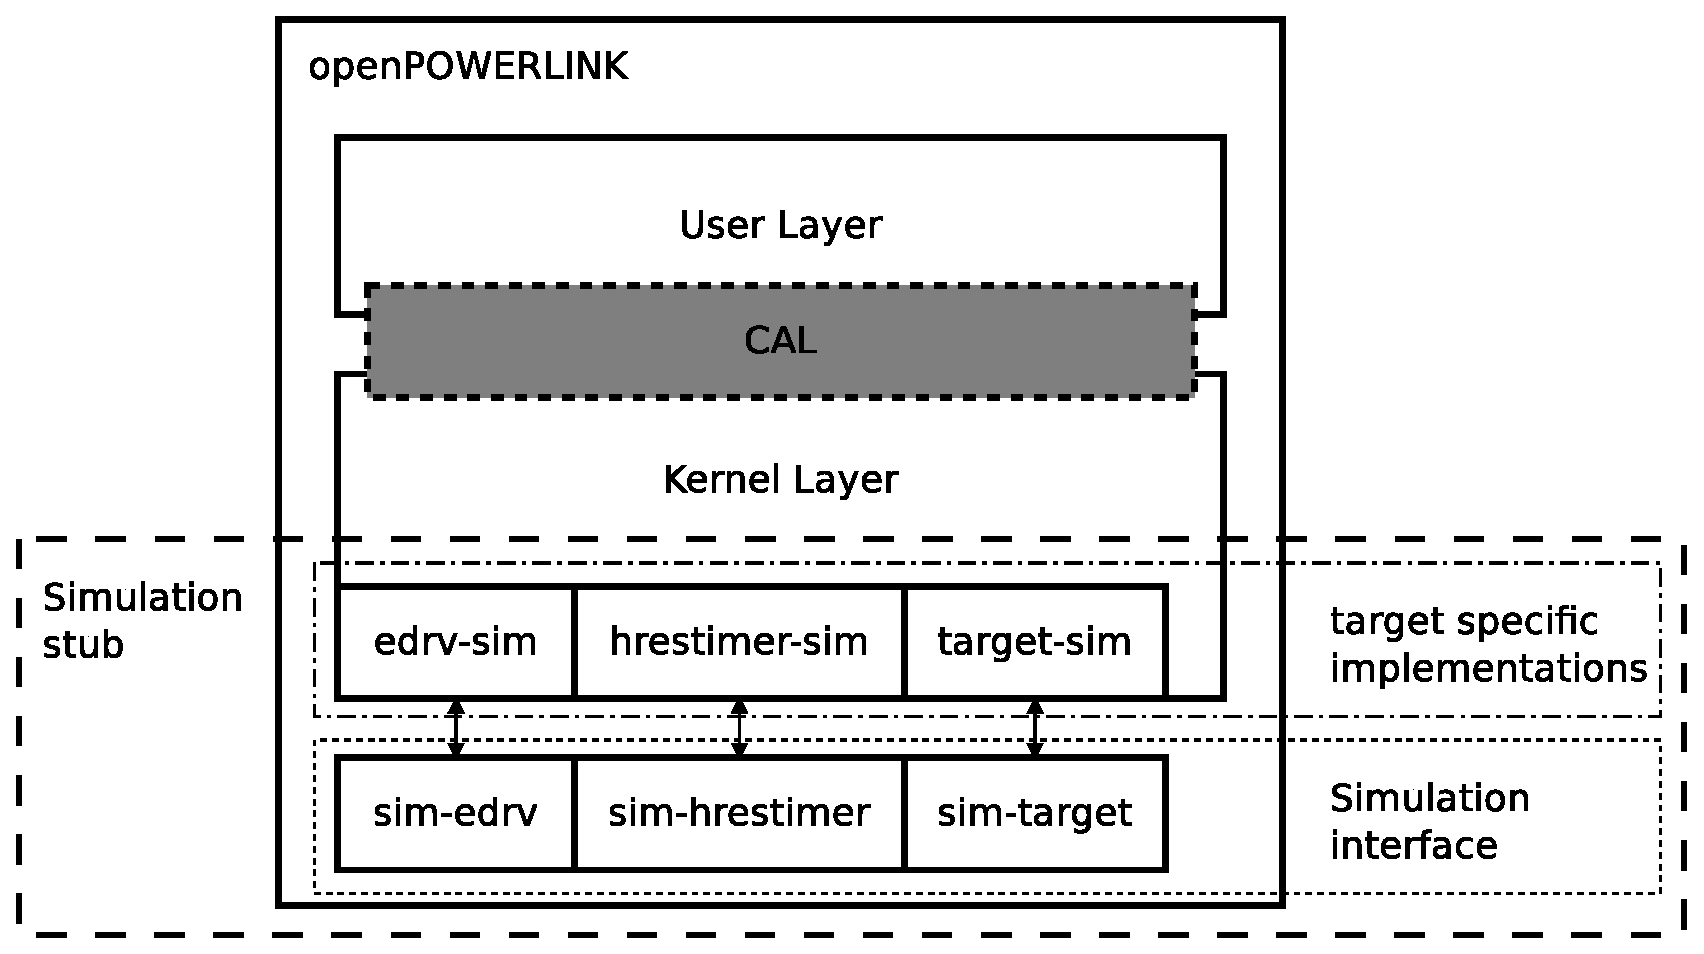
\includegraphics[width=0.9\linewidth]{simulation_stub}
    \caption{Example hierarchy of the simulation stub (dashed, left) and the included target specific implementation (dash-dottet, right) and simulation interface (dashed, right).}
    \label{fig:simulation_stub}
\end{figure}

For minimizing the necessary changes in the openPOWERLINK stack the simulation stub is separated into two components the specific implementations for the \emph{sim} target and the simulation interface.
An example hierarchy of the simulation stub is shown in figure \ref{fig:simulation_stub}.
The enclosed target specific implementations and the simulation interface are explained in the following sections.

\subsection{Target specific implementation}
\label{sec:porting_simstub_target}

Similar to the specific implementations for various modules in the openPOWERLINK stack (as described in section \ref{sec:oplk_architecture}) the implementations for the \emph{sim} target were added as specific implementations of the given common header files.
As shown in figure \ref{fig:simulation_stub} the target specific implementations are embedded in the kernel layer of the openPOWERLINK stack.

\begin{sloppypar}
The appendix section \ref{app:simulation_edrv_target} shows the implementation of the \emph{edrv\_sendTxBuffer} function from the \emph{edrv-sim} implementation.
\end{sloppypar}

Within the target specific implementations of different modules only function calls to the simulation interface and small parameter conversions are implemented.
The simulation interface is located in a newly introduced folder named \emph{sim}.
The content of this folder and the targeted purpose is shown in the next section.

\subsection{Simulation interface}
\label{sec:porting_simstub_siminterface}
The \emph{sim} folder contains two main folders separating the source and include files.
Each module within the openPOWERLINK stack, which should be connected to the simulation environment, has its specific simulation module within the simulation interface.
The naming of the different simulation interface modules shows the common prefix \emph{sim} separated with a hyphen from the implemented module name.
The connection between the target specific implementation and the simulation interface is shown in figure \ref{fig:simulation_stub}. 

\begin{sloppypar}
The simulation interface contains all functions which are required by the ported stack module.
Additionally each simulation interface provides a set<\emph{ModuleName}>Functions function.
For all functions which should be connected to the simulation an according function pointer is defined as typedef and all functions are grouped in a structure named t<\emph{ModuleName}>Functions.
For a common include file containing all types required for the simulation interface the typedefs for each function pointer and the structures are defined within the header file \emph{sim.h}.
This structure is passed to the set<\emph{ModuleName}>Functions function and its content is checked for validity.
Only when all of them are valid the structure is saved in the static instance and a flag is set for valid initialization.
\end{sloppypar}

When a function of the simulation interface is called by the stack the stored static instance is checked and the according function is called.
Therefore the external functions are called and the connection from the stack to the simulation environment is established.

For configuring the simulation interface from the simulation environment, the accessible function set<\emph{ModuleName}>Functions is declared as an exported function for shared libraries.
This is done via the preprocessor macro \emph{OPLKDLLEXPORT} defined by the openPOWERLINK stack.
This macro is defined within the target specific includes located in \emph{stack/include/oplk/targetdefs} as described in section \ref{sec:oplk_platform_hardware} and marks the exported functions for the shared library.

The appendix section \ref{app:simulation_edrv} shows the definition and implementation of the simulation interface module \emph{edrv-sim} regarding the initialization and the sendTxBuffer function as example.
As shown in the appendix an additional parameter was added to each function.
This is necessary for supporting the simulation of multiple openPOWERLINK stack instances within a single simulation.
The used strategy is described in section \ref{sec:porting_stack_multiinstance}.

For the opposite direction of calling a stack function from the simulation environment two cases are distinguished.

\begin{enumerate}
    \item Is the desired function already an exported function, e.g. a part of the public \emph{API}, it is resolved and called directly from the simulation environment.
    \item Is the desired function not exported an according function in the simulation interface module must provided.
    Within the implementation of such a function the according stack function can be called directly.
\end{enumerate}

In both cases no target specific implementation is required, because no implementation is replaced by the simulation, only additional functions are made accessible.

The connection of the openPOWERLINK stack to the simulation environment is designed independently of OMNeT++ and does not require any OMNeT++ functionalities.
This independence was established for supporting various simulation environments and systems.
The simulation interface can be used by every application and simulation environment which is capable of handling a native shared libraries and function pointer.

For this paper the simulation environment OMNeT++ was chosen and the modified openPOWERLINK stack is embedded in an OMNeT++ simulation.
The following sections show the implementation of the simulation and its different components.

\section{Simulated stack}
\label{sec:porting_stack}
The simulated stack consists of the five implemented modules \emph{edrv}, \emph{hrestimer}, \emph{target}, \emph{sdoudp} and \emph{trace}.
These modules will also be implemented as simple modules representing the simulated structure and functional units.

The result of the successful build process of the modified openPOWERLINK stack is a shared library exporting the by default exported functions and new functions for interacting with the simulation interface.
The structure of the developed simulation and the enclosed components are described in the following section.

\subsection{Simulation structure}
\label{sec:porting_stack_simstructure}
Within the openPOWERLINK simulation the fundamental folder structure is taken from OMNeT++ recommendations and separates the simulation configuration (\emph{simulations} folder) from the implemented model (\emph{src} folder).
For better representation of custom openPOWERLINK nodes the \emph{images} folder contains customized icons with an embedded openPOWERLINK logo.

The implemented model within the \emph{src} folder is separated in different folders for the \emph{MN}, the \emph{CN} and a generic node implementation.
These nodes and the implemented hierarchy is described in the section \ref{sec:porting_nodes}.

Approaching the counterpart to the above described simulation interface the generic node contains a \emph{stack/interface} folder containing the implementation of the interface to the simulated openPOWERLINK stack.
The functionalities and the underlying strategy of this interface implementation is described in the following section.

\subsection{Interface Implementation}
\label{sec:porting_stack_interface}
The implementation of the interface within the simulation is based on the usage of the following two classes providing the basic functionalities for handling the connection to the simulation interface.

\emph{OplkBase} represents a base class for every interface module connected to the simulated openPOWERLINK stack.
It is implemented as a template class taking a template type for a module.
This module is grouped together with an instance of the second class \emph{SharedLibraryHelper}.
The class diagram containing \emph{OplkBase}, \emph{SharedLibraryHelper} and as example the implemented classes \emph{Edrv} and \emph{OplkEdrv} are shown in figure \ref{fig:simulation_stack_interface_classes}.

\begin{figure}
    \centering
    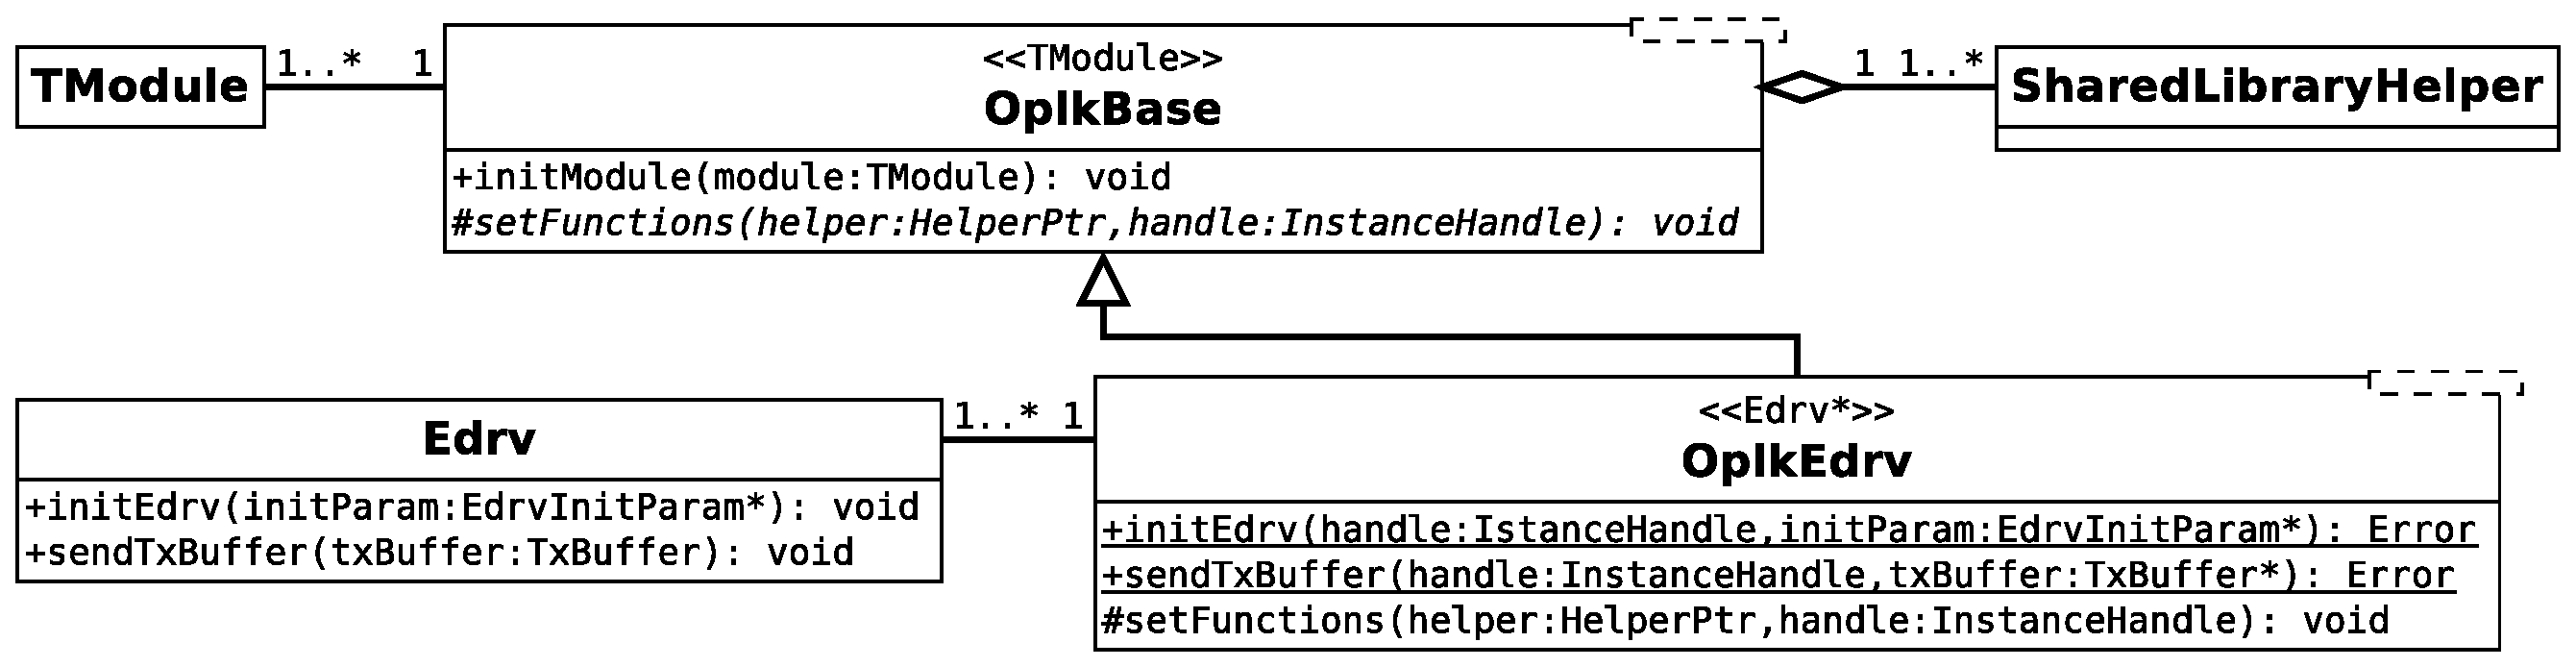
\includegraphics[width=0.9\linewidth]{simulation_stack_interface_classes}
    \caption{Class diagram showing the inheritance used for the stack interface.}
    \label{fig:simulation_stack_interface_classes}
\end{figure}

The class \emph{SharedLibraryHelper} is implemented independently of the OMNeT++ framework and provides methods for the handling of an shared library.
The internal implementations are defined by preprocessor macros and results in according implementations for Linux and Windows.
Basically the \emph{SharedLibraryHelper} allows the loading of a defined shared library object and the resolving of defined functions.
The shared library is opened during creation of an \emph{SharedLibraryHelper} and is closed during destruction
Thereby this class follows the design principle of Resource Acquisition Is Initialization (RAII).
This ensures the correct closing of all opened shared libraries during shutdown and prevent possible resource leaks.
The resolved functions are returned as std::function objects with the requested types.
The usage of functional objects instead of simple function pointer allows more dynamic handling within the object oriented environment.

The class \emph{OplkBase} provides a \emph{initModule} method taking an instance of the template type as parameter (as shown in figure \ref{fig:simulation_stack_interface_classes}).
This function creates a new instance of \emph{SharedLibraryHelper} with the internally saved library name and stores the helper object together with the given module in an internal container.

After this creation the helper object and the index of the currently added instances within the internal container is passed to the method \emph{setFunctions}.
This method is defined pure virtual and demands the implementation by a derived class.

Via deriving from \emph{OplkBase} all implemented interface classes contains the functionality of holding the according \emph{SharedLibraryHelper} with an instance of the defined module type.
These derived classes are named according to the implemented module with \emph{Oplk} as prefix and located within the \emph{interface} folder and the \emph{interface} C++ namespace.
The template parameter is mostly defined as pointer to the according OMNeT++ module which is named simple by the implemented module, e.g. \emph{Edrv} represents the OMNeT++ module for the Ethernet driver module.
The described inheritance and connection is shown in figure \ref{fig:simulation_stack_interface_classes}.

This connection of \emph{SharedLibraryHelper} and the module instance is demanded by the requirement for multiple simulated instances of the openPOWERLINK stack within a single simulation.
This requirement, its consequences, the solution and the implementation are described in the next section.

\subsection{Multiple instances}
\label{sec:porting_stack_multiinstance}
The openPOWERLINK stack is designed as pure ANSI C implementation structured in multiple modules.
The designated usage of the openPOWERLINK stack is the execution on devices representing a single node.
Because of this designated usage no demand for multiple instances is given and the informations about various states, buffer and all other data are stored within the openPOWERLINK stack as static variables.
These variables exist once in the compiled application or library.
Therefore the simulation of multiple instances within a single application by normally linking to a shared or static library is not possible.

The solution for this problem is the loading of the same shared library multiple times in a manner that the loaded library exists multiple times within the memory.
Linux supports the loading of a single shared library multiple times into the memory and therefore creating multiple instances unfortunately Windows does not provide such a functionality.
OMNeT++ is supporting Windows and Linux in the same way and for achieving a simulation which is usable in the identical way on either Linux or Windows another strategy has to be found.

When the binary file of a shared library is copied and named differently both files can be loaded into the memory as different libraries.
This strategy does not require any special functionality and can be implemented for Windows and Linux in the same way.
This handling of multiple shared libraries and the copying of the binary file on demand is implemented by the \emph{SharedLibraryHelper}.
Starting with the manually created instance any further instances can be accessed by the method \emph{getNextLibrary} which copies the shared library if necessary and creates a new instance with the copied library file.
When a new instance is requested but the maximum number of allowed instances is exceeded an exception is thrown.
When not caught otherwise this exception would cause the simulation to shutdown and according information is presented to the user.


\subsection{Instance association}
\label{sec:porting_stack_instance_assoc}
As mentioned in section \ref{sec:porting_simstub_siminterface} and shown in appendix section \ref{app:simulation_edrv} the simulation interface includes an instance handle parameter.
This handle is passed when the set<\emph{ModuleName}>Functions function of an interface module is called and is stored in the static instance information within the simulation interface module.
When a function call from the openPOWERLINK stack is forwarded to the simulation interface the stored handle is passed to the called function pointer.
The counterpart within the stack interface can then assign the function call to a specific instance.
This assignment is done within the derived classes of \emph{OplkBase}.
The derived classes must be implemented as singleton and therefore support only a single instance within the application.
This instance holds the container of modules (given via the method \emph{initModule}) and assigned \emph{SharedLibraryHelper} instances.
The passed instance handle represents the index within this internal container and is created after inserting the instances within the \emph{initModule} method of \emph{OplkBase}.
This structure and the quantity of the different modules is shown in figure \ref{fig:simulation_instances}.

The pure virtual method \emph{setFunctions} of \emph{OplkBase} must be implemented by a derived class and gets the \emph{SharedLibraryHelper} instance and the associated instance handle as shown in  figure \ref{fig:simulation_stack_interface_classes}.
Within this method each derived class must initialize the demanded functions and connections to the simulation interface.
This is done by optional creating an according structure of function pointers pointing to static methods.
After successful resolving of the set\emph{ModuleName}Functions function this structure with the assigned handle is passed to the according simulation interface.

When a function call is forwarded from the openPOWERLINK stack over the simulation interface to the static method the stored instance handle is passed as parameter.
This handle can be used for getting the according module instance from the internal container of modules and \emph{SharedLibraryHelper} instances.
The according method can be called using the stored module instance.

For the opposite direction of communication the \emph{setFunctions} method can be used for resolving the required functions from the simulation interface using a specific shared library instance and saving them in the given module instance.
When calling one of this stored functions the correct shared library instance is used due to the previous resolving of all functions.

An overview of this hierarchy and the connections of different instances is shown by an exemplary composition in figure \ref{fig:simulation_instances}
The shown example includes the OMNeT++ environment an the bottom containing two instantiated nodes.
The \emph{MN} and the \emph{CN} represent separate simulated nodes within an POWERLINK network.
Each node contains an \emph{edrv} instance which is registered as module within in the \emph{oplkEdrv} instance.
Above the OMNeT++ environment two openPOWERLINK stacks are shown, which exists independently of each other.
Each openPOWERLINK stack contains the simulation interface module \emph{sim-edrv} and the target specific implementation \emph{edrv-sim}.
The two stacks connected to the two nodes demonstrate the two directions of function calls.

The left side including the \emph{MN} is called by the openPOWERLINK stack forwarding the function call from the \emph{edrv-sim} to the simulation interface \emph{sim-edrv}.
This adds the internally stored handle to the parameters and calls the saved static method of \emph{oplkEdrv}.
Using the passed handle the according module instance \emph{edrv 0} is accessed and the according function is called.
The shown dashed arrows mark the path of the according return values.

The right side including the \emph{CN} requests the function object for a specific function of \emph{sim-edrv} within stack 1.
The \emph{SharedLibraryHelper} instance saved in \emph{oplkEdrv} returns the correct function object.
This is called by \emph{edrv 1} and therefore the function of \emph{sim-edrv} is directly invoked.
This call is then forwarded to the openPOWERLINK stack directly within \emph{sim-edrv}.

\begin{figure}
    \centering
    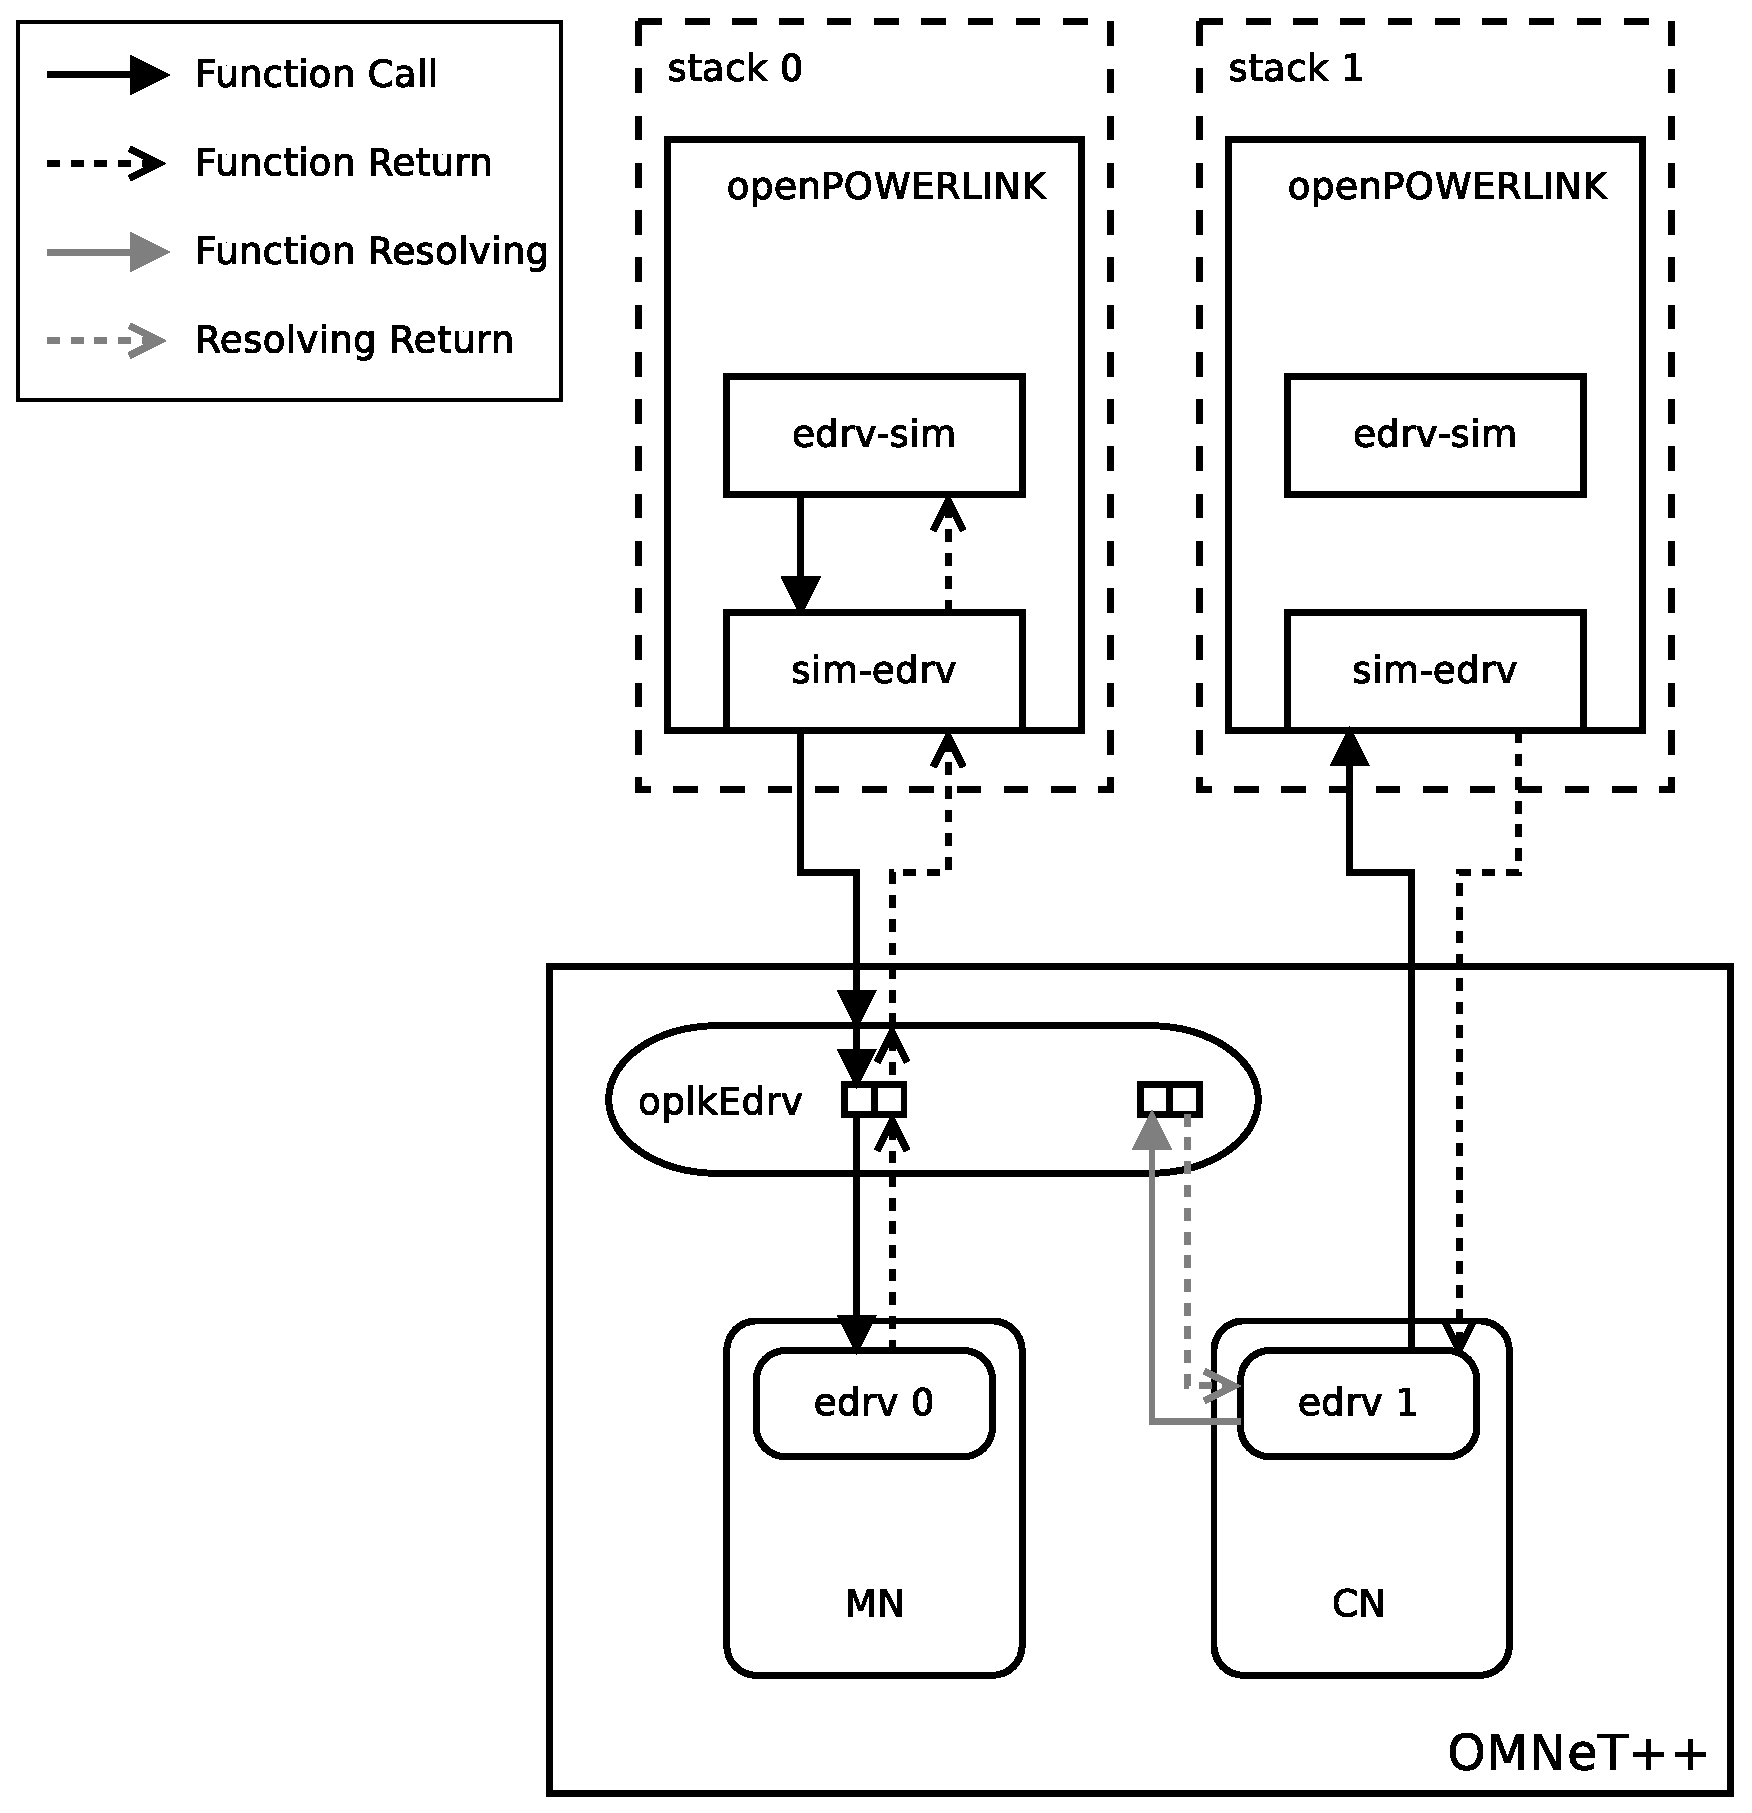
\includegraphics[width=0.7\linewidth]{simulation_instances}
    \caption{Hierarchical overview of the simulation environment, embedded modules the stack interface and simulation interface.}
    \label{fig:simulation_instances}
\end{figure}

The implementation of \emph{OplkBase}, \emph{SharedLibraryHelper} and \emph{OplkEdrv} are shown in appendix section \ref{app:simulation_stackif}.
In appendix section \ref{app:simulation_sim_edrv} the implementation of \emph{Edrv} is shown.

The further implementation and structuring of the according OMNeT++ modules is described in the following section.

\subsection{Stack module}
\label{sec:porting_stack_stackmodule}

The previous mentioned OMNeT++ modules representing components within the openPOWERLINK are located in the \emph{stack} folder.
Additionally to the platform dependent modules the \emph{Api} module was implemented providing all functions exported by the openPOWERLINK \emph{API}.
These modules provide the functions which implement the required functionalities for the openPOWERLINK stack.
The combination of these modules illustrate a single openPOWERLINK stack module and represent a single openPOWERLINK stack instance which is shown in figure \ref{fig:simulation_stack_module}.

\begin{figure}
    \centering
    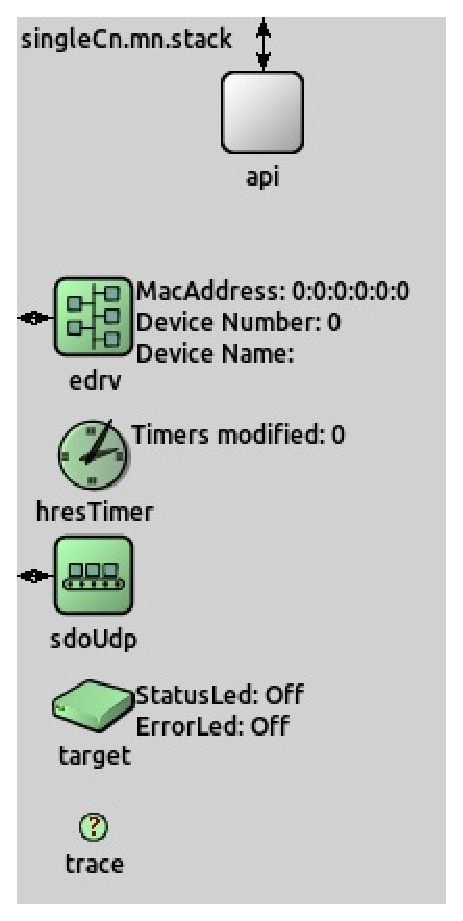
\includegraphics[width=0.35\linewidth]{simulation_stack_module}
    \caption{Composition of compound module representing the openPOWERLINK stack.}
    \label{fig:simulation_stack_module}
\end{figure}

The different modules implement the required functionalities using OMNeT++ functionalities, e.g. scheduling self messages for implementing the timer functionality.
The \emph{Edrv} and the \emph{Sdoudp} modules define input and output gates transmitting and receiving the according data.
The \emph{Api} also provides gates for receiving a command defining a specific \emph{API} function which should be invoked.
Occurring events and resulting return values are sent within messages by the \emph{Api} module via the according gates.

The compound module shown in figure  \ref{fig:simulation_stack_module} represents a single stack instance.
For the usage of the stack instance the combination with an application is necessary.
This combination is implemented within the compound module \emph{GenericNode} providing the common functionalities for \emph{MN} and \emph{CN}.
The different implemented nodes are described in the following section.

\section{Simulated nodes}
\label{sec:porting_nodes}
Analyzing different demo applications included in the openPOWERLINK stack distribution package a general structure can be determined including the following modules.

\begin{description}
    \item[main/demo] The implementation of the main application handles the initialization, the main loop and the shutdown procedure for the demo application.
    \item[app] The app module contains the handling of application specific operations, i.e. the creation of the process image and the according synchronized procedure for modifying the process image.
    \item[event] The event module handles all occurring events coming from the openPOWERLINK stack.
\end{description}

The implementation of the nodes located within the \emph{generic} folder should provide a basic functionality allowing a simple environment for fast development of an demo application.
Therefore this structure was implemented within the \emph{GenericNode} using base classes for each module as described in the following section.

\subsection{Generic node}
\label{sec:porting_nodes_generic}
All implementations regarding the generic functionalities of a simulated node are located in the \emph{generic} folder.
The compound module \emph{GenericNode} contains an instance of the \emph{Stack} module and modules defined by the interfaces \emph{IDemo}, \emph{IEvent} and \emph{IApp}.
These interfaces represent the defined structure of every node.
The defines gates of each module are necessary for the base implementation and its functionalities.

This implementation is represented by the base classes \emph{DemoBase}, \emph{EventBase} and \emph{AppBase}.
Their implementations contain default message handling, resolving of the defined gates or parameters and statistics recording.

The designated usage of these base classes is deriving a specialized class for each specific node.
These derived classes can be inserted within the \emph{GenericNode} by setting the according parameter.
The parameter \emph{DemoType}, \emph{EventType} and \emph{AppType} are defined in \emph{GenericNode} and are used for the insertion of the derived \emph{Demo}, \emph{Event} and \emph{App} module.

The implementation of the \emph{GenericNode}, the used moduleinterfaces and the base classes for each module are shown in the appendix sections \ref{app:simulation_sim_generic}, \ref{app:simulation_sim_moduleinferfaces}, \ref{app:simulation_sim_baseclasses}.

The composition of the \emph{GenericNode} connecting the embedded \emph{Stack} module and instances matching the different moduleinterfaces is shown in figure \ref{fig:simulation_genericnode}.

\begin{figure}
    \centering
    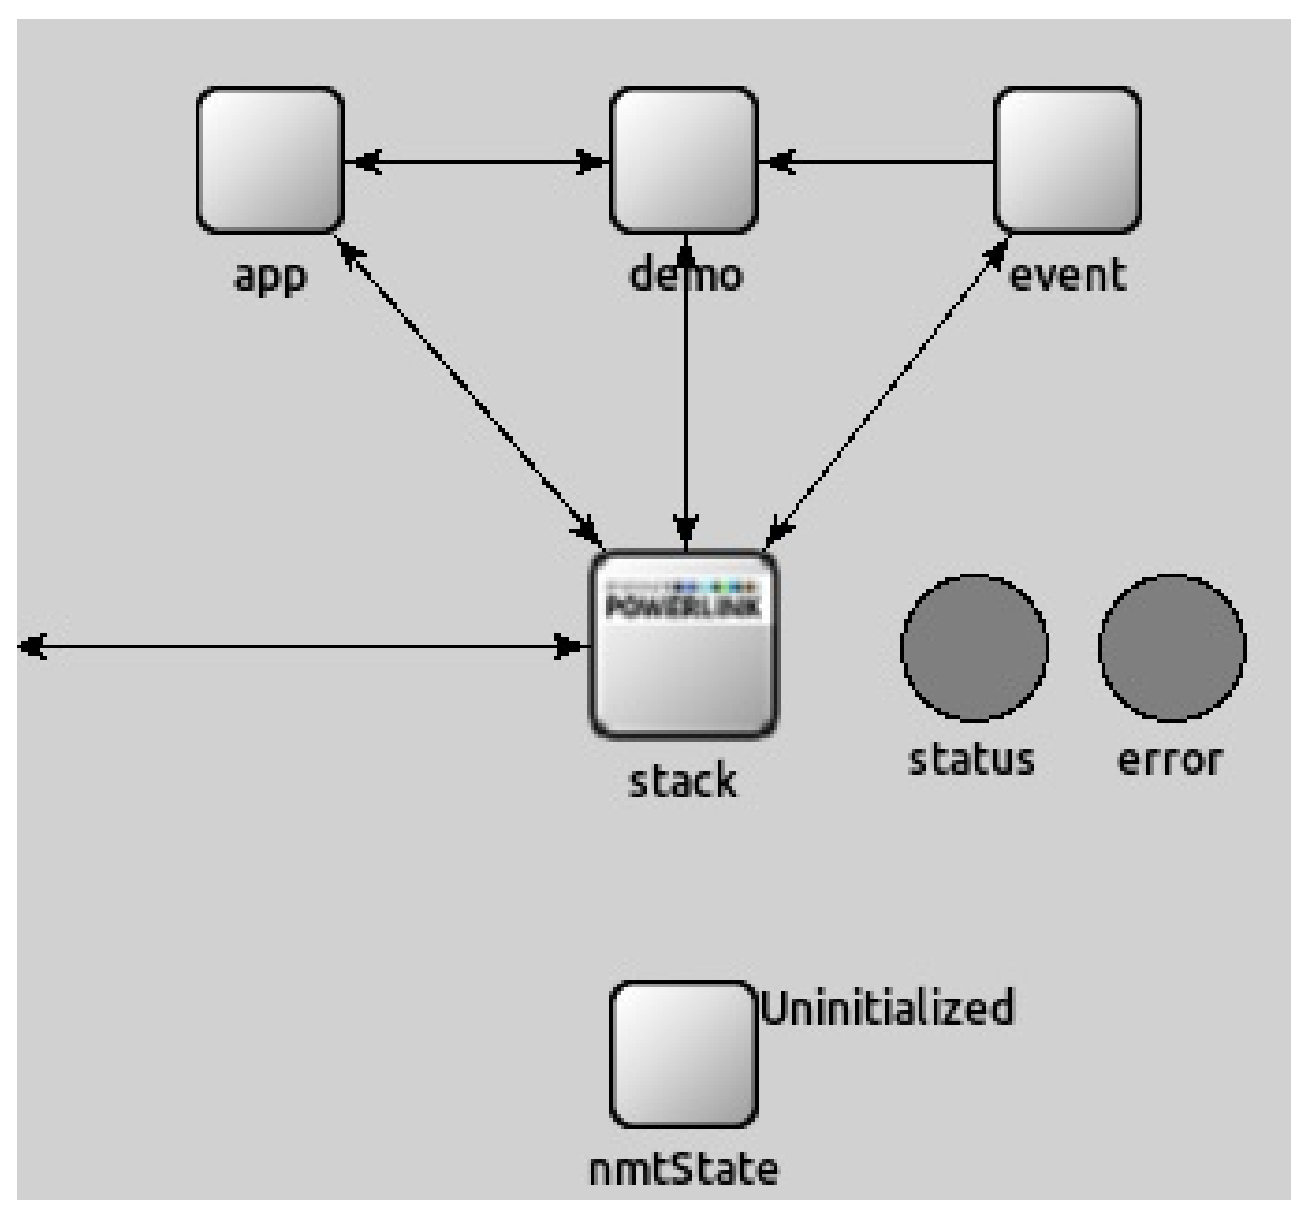
\includegraphics[width=0.35\linewidth]{simulation_genericnode}
    \caption{Composition of compound module representing the a generic openPOWERLINK node.}
    \label{fig:simulation_genericnode}
\end{figure}

For a convenient display of the current state of the node the additional module \emph{NmtState} was implemented and added to the \emph{GenericNode}.
This module does not support any communication via messages, but it subscribes to a signal of its parent module.
The name of the signal can be configured via a parameter, which is set to the default value \emph{nmtState} (defined signal of \emph{EventBase}).
when an notification for this signal is available the received unsigned long value is casted to an NmtState and the according string is displayed.

The \emph{GenericNode} is designed for deriving and extending its functionality for specific nodes and applications.
The functionality of a \emph{MN} and \emph{CN} must be implemented separately as shown in the next sections.

\subsection{\emph{MN} and \emph{CN}}
\label{sec:porting_nodes_mn_cm}
The implementation of the \emph{MN} was achieved by analyzing and porting the \emph{demo\_mn\_console} and the \emph{demo\_mn\_embedded} to the OMNeT++ simulation.
Both demo applications were analyzed for achieving the correct implementation of the simulated \emph{MN}.

The \emph{MN} folder within the \emph{src} directory contains the module definition of the \emph{MN} module and the specific derived classes \emph{MnDemo}, \emph{MnEvent} and \emph{MnApp}.
These classes implement the according functions of the base classes described in section \ref{sec:porting_nodes_generic}.
This folder and the contained implementations can be used as base project for further implementations using a simulated \emph{MN}.

Similar to the implementation of the \emph{MN} contains the \emph{CN} folder the according module definitions and implementation for achieving the functionality of a \emph{CN}.

The different implemented classes could either be replaced by alternative implementations of the moduleinterfaces or derived classes from the base classes.
Or the classes are used as base classes and any further functionality is embedded.
This extension is easily possible due to the virtual definition of all used methods.
\\

The results of running the openPOWERLINK simulation consisting of a \emph{Mn} connected to a single \emph{CN} are shown in the next chapter.